\chapter{Characterization: How we measured the actual grating performance, and accounted for differences}

\section{AFM measurements of manufactured grating profile}

\begin{figure}[htbp] %  figure placement: here, top, bottom, or page
   \centering
   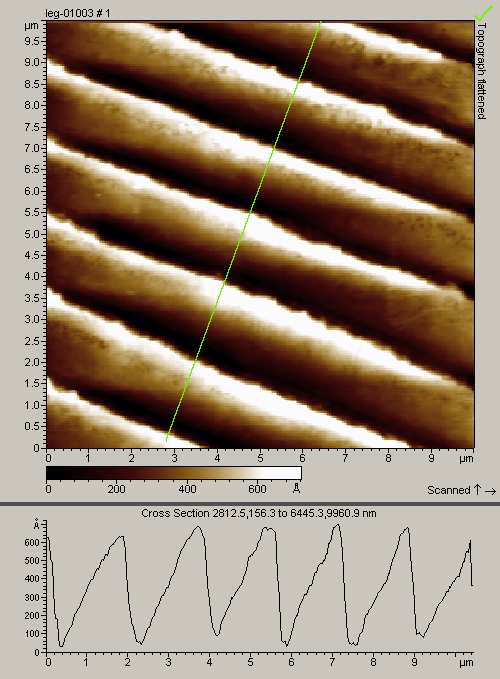
\includegraphics[width=6.5in]{Chapter5/5a_exampleAFM/afm_LEG_xsect1.png} 
   \caption{The Low Energy Grating has a smooth regular profile, shown in this example image measured using an Atomic Force Microprobe (AFM).}
   \label{5a}
\end{figure}


[locate all]

challenge: blaze angle numerical measurements... requires calibration of z-axis.

\section{Diffractometer measurements of actual grating efficiency}

\subsection{Beamline 6.3.2 Diffractometer}
- describe machine

TODO: get paper and cite: http://ieeexplore.ieee.org/xpl/freeabs\_all.jsp?arnumber=4994440

\begin{figure}[htbp] %  figure placement: here, top, bottom, or page
   \centering
   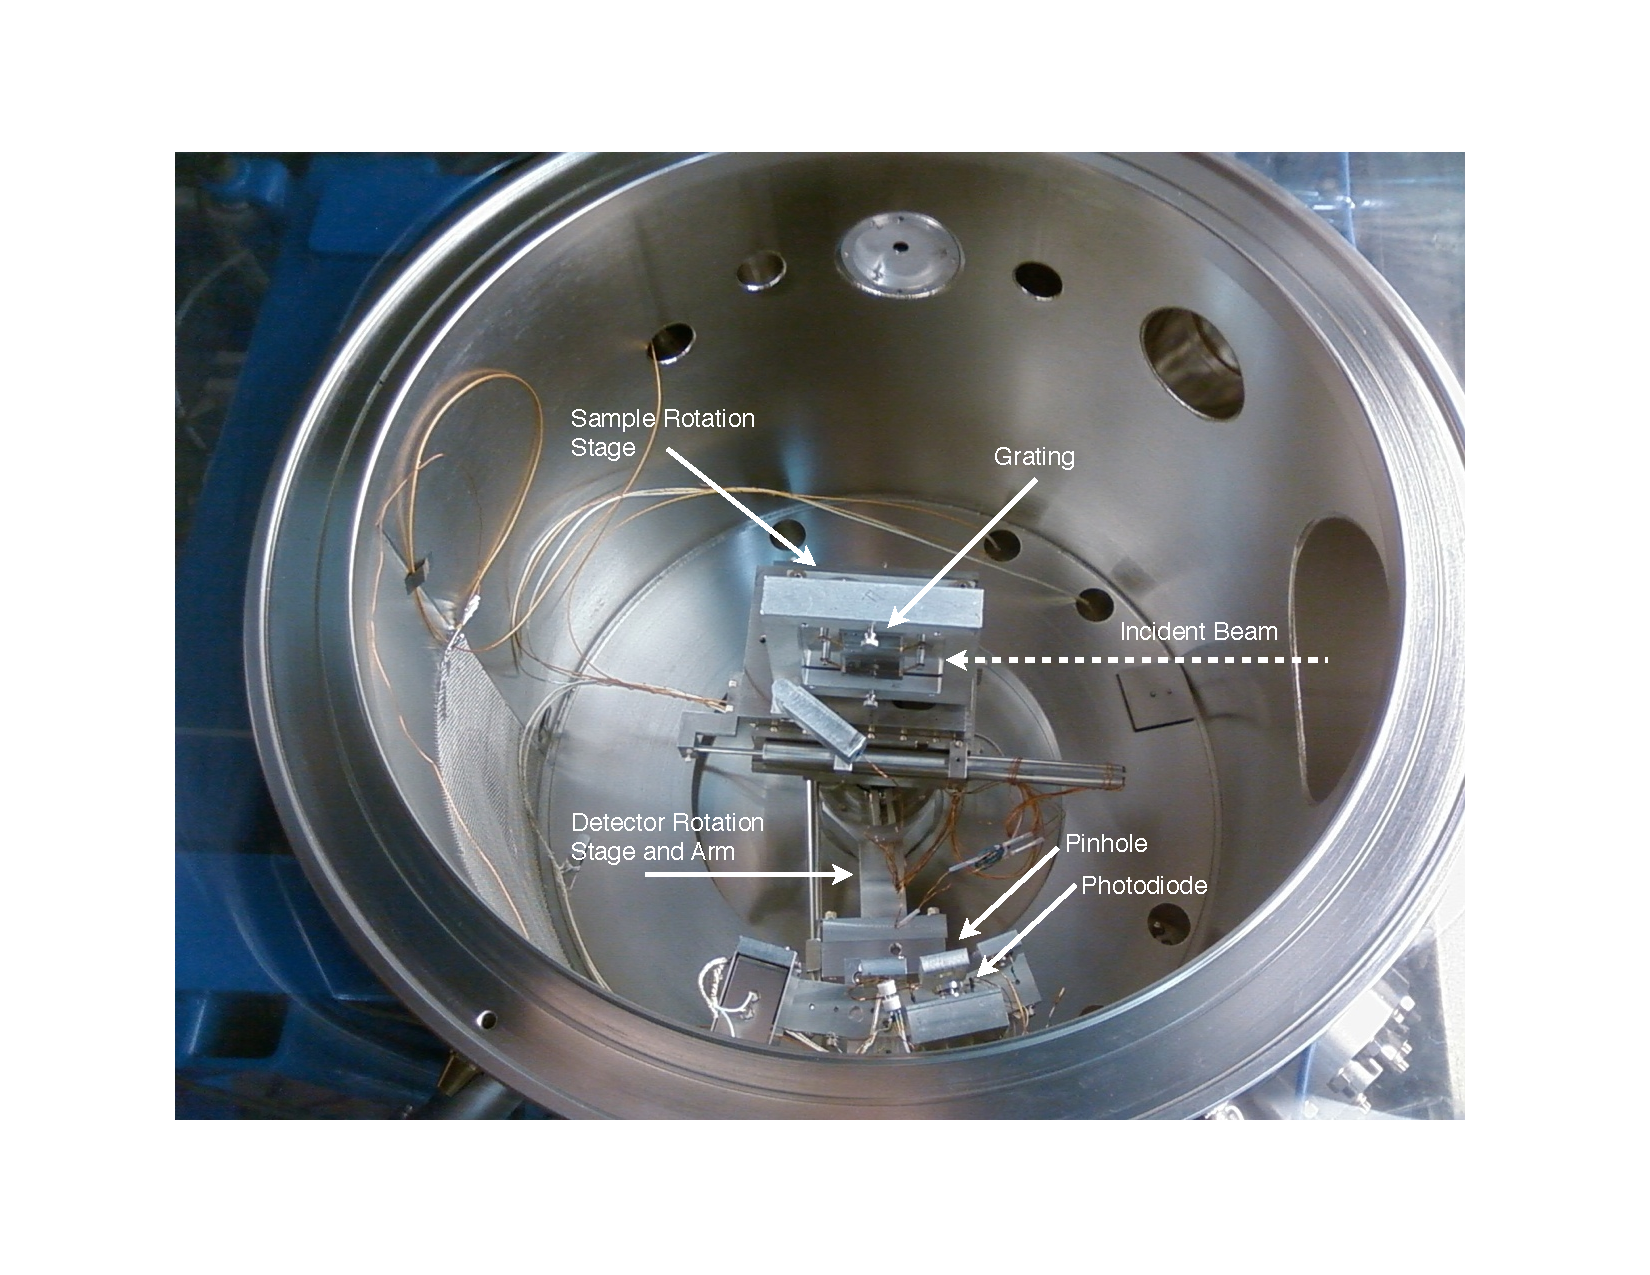
\includegraphics[width=7in]{Chapter5/5b_diffractometer/diffractometer_labelled.pdf} 
   \caption{The diffractometer on Beamline 6.3.2 at the Advanced Light Source allows for independently setting the angle of the gratings in the beam, and setting the angle of a pinhole photodiode detector.  Upstream, filters in the beamline are used to remove contamination from the higher-order light of the monochromator. }
   \label{5b}
\end{figure}

FIGURE 5b: picture of diffractometer tank with gratings positioned

- If you know groove density: can position to detector to correct angle as you scan energy. Otherwise, need to scan angle to find diffraction peak, and take eff. there.

DATA 5c: example angle scan at energies of interest

\begin{figure}[htbp] %  figure placement: here, top, bottom, or page
   \centering
   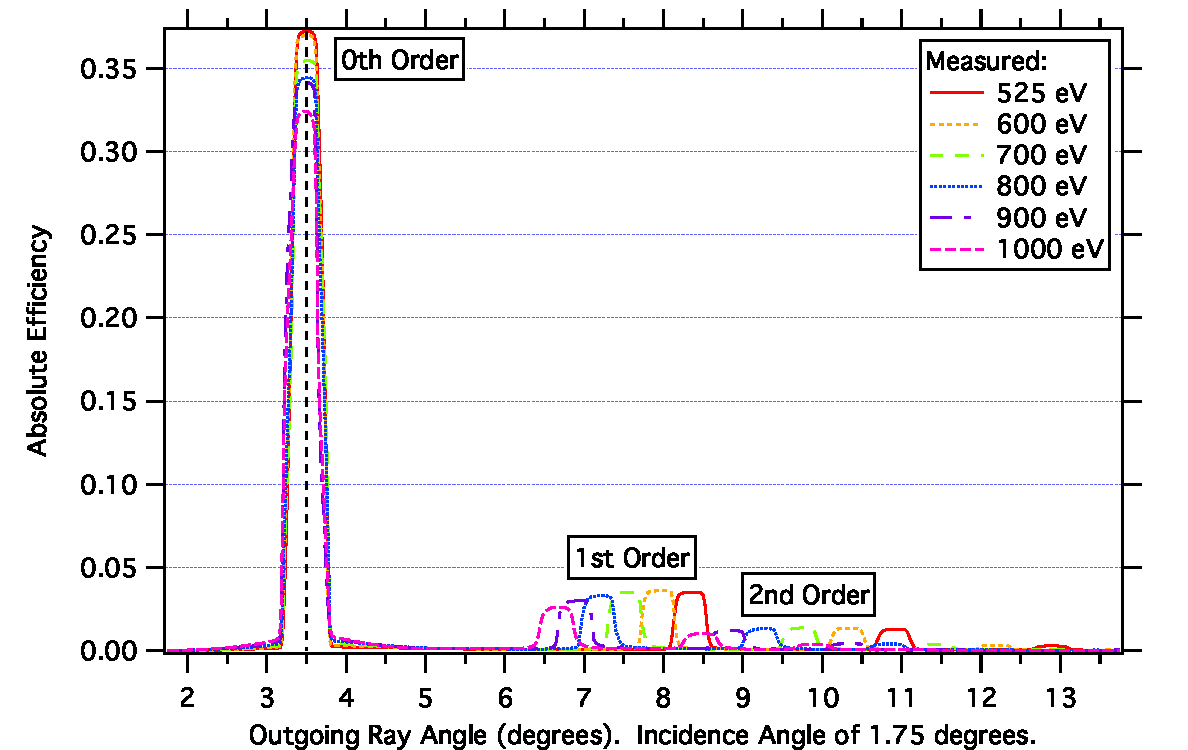
\includegraphics[scale=0.8]{Chapter5/5c_angleScan/5c.pdf} 
   \caption{The simplest diffractometer experiment scans the detector angle while illuminating the grating with a constant photon energy.  The diffraction orders are visible as peaks along the outgoing angle axis (here, measured up from the grating surface at 0 $\deg$).  The 0th order (reflection) peak is easily visible at twice the incident angle.  (Grating: HRHEG)}
   \label{5c}
\end{figure}

DATA: 5d example energy scan known groove density

\begin{figure}[htbp] %  figure placement: here, top, bottom, or page
   \centering
   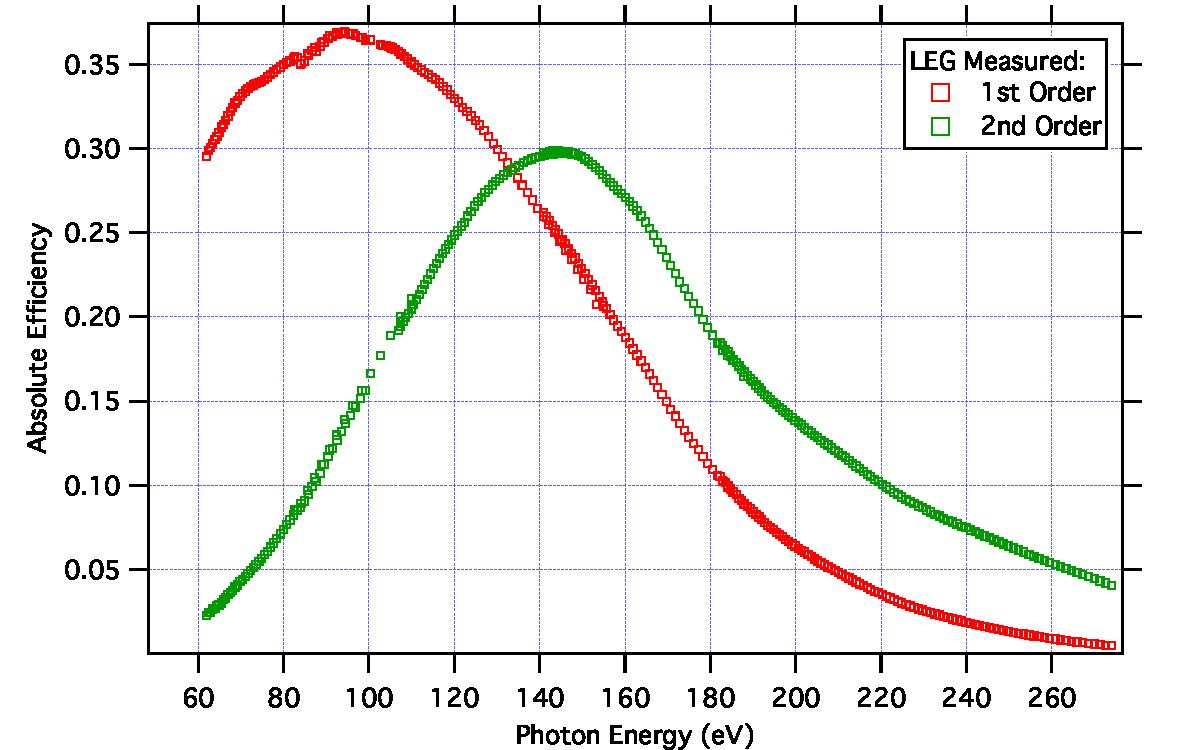
\includegraphics[scale=0.8]{Chapter5/5d_energyScan/5d_LEG.pdf} 
   \caption{When the groove density of a grating is accurately known, the detector angle can be scanned in synchronization to keep it on the diffraction peak as the incident photon energy is scanned.  This allows faster, continuous efficiency measurements as a function of  photon energy.  (Grating: LEG)}
   \label{5d}
\end{figure}

- mono: higher-order light contamination.  Uses filters in front of end station

\section{Real-world grating effects}
\label{realWorldEffects}
\subsection{Stray Radiant Energy}
http://gratings.newport.com/information/technotes/technote9.asp
\subsubsection{Surface roughness}
 (scattering: uniform decrease in efficiency)
  Other way to think about: periodic structures with \emph{many} frequency components. Diffract all over the place.
  
  TODO: Find reference and descriptive math...
  
          - Not modelled.  Accept a uniform constant reduction (usually about ~50\%) lower due to scattering.

\begin{figure}[htbp] %  figure placement: here, top, bottom, or page
   \centering
   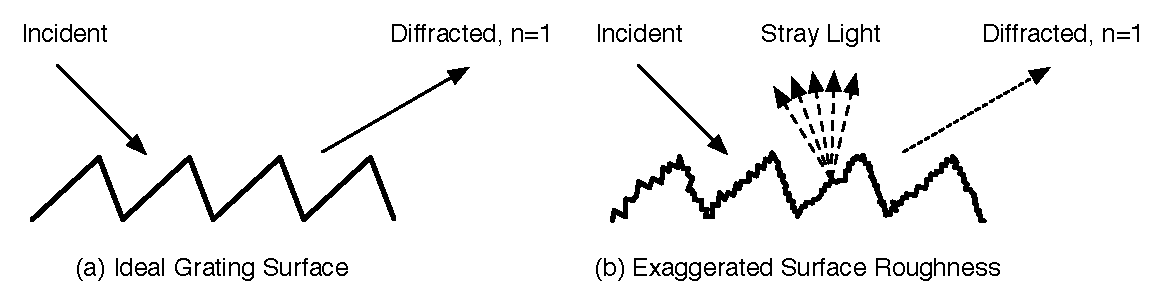
\includegraphics[scale=0.8]{Chapter5/5e_surfaceRoughness/5e.pdf} 
   \caption{Roughness of the grating surface scatters stray light outside the diffraction orders}
   \label{5e}
\end{figure}
       

\subsubsection{Dust, scratches, pinholes act as scattering centers}
\subsubsection{Irregularities in the groove position create ghost peaks}
\subsubsection{Irregularities along the groove direct light elsewhere}
reflect off axis... reduce periodicity... disrupt the perfect grating model. May be directed or diffuse.
\subsection{Blaze angle errors shift the efficiency peak}
\subsection{Coating oxidation changes the reflectivity spectrum}

\begin{figure}[htbp] %  figure placement: here, top, bottom, or page
   \centering
   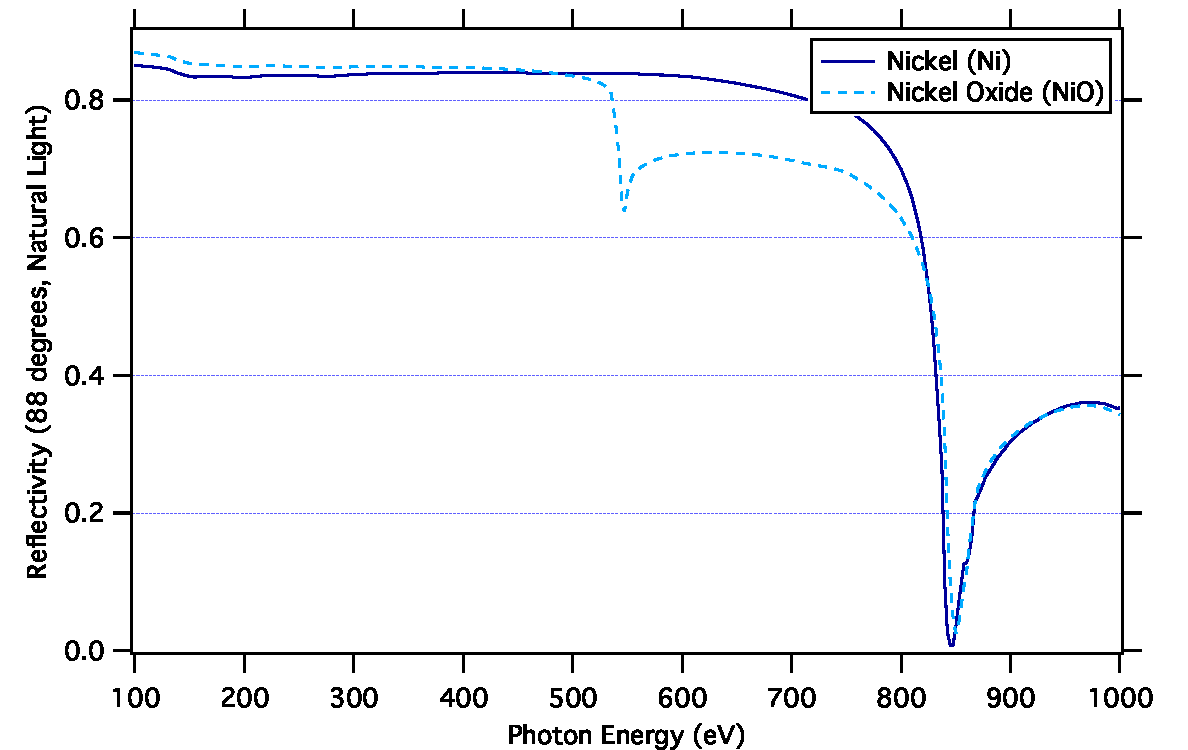
\includegraphics[scale=0.8]{Chapter5/5f_oxidized/Ni_NiO_reflec.pdf} 
   \caption{Unprotected Nickel quickly forms a surface oxide of NiO, which strongly reduces the reflectivity at the Oxygen edge (525eV) }
   \label{5f}
\end{figure}

\section{Grating results}
   : (and comparison to theoretical)
\subsection{LEG} (gold): profile clean; as expected; blaze angle off. [modelled]

\begin{figure}[htbp] %  figure placement: here, top, bottom, or page
   \centering
   \includegraphics[scale=0.8]{Chapter5/5y_afm/LEG.pdf} 
   \caption{AFM measurements of the Low Energy Grating (LEG) profile, averaged along the grooves (TODO um x TODO um).  The best-fit blaze angle is at the centre of the grating.}
   \label{5y-leg}
\end{figure}

\begin{figure}[htbp] %  figure placement: here, top, bottom, or page
   \centering
   \includegraphics[scale=0.8]{Chapter5/5x_comparison/LEG.pdf} 
   \caption{Theoretical and measured efficiency of the Low Energy Grating (LEG).}
   \label{5x-leg}
\end{figure}


\subsection{IMP} (nickel): Profile clean, blaze angle off [modelled].  Oxidized� Modelled as NI, layer of NiO.

TEST: NiO on top of Ni? layer thickness
Caveat: Henke data reflectivities are not correct at/near absorption edges... shouldn't totally match theoretical shape.

          - compare AFM and fitted

\begin{figure}[htbp] %  figure placement: here, top, bottom, or page
   \centering
   \includegraphics[scale=0.8]{Chapter5/5y_afm/IMP.pdf} 
   \caption{AFM measurements of the Impurity Grating (IMP) profile, averaged along the grooves (TODO um x TODO um).  The best-fit blaze angle is at the centre of the grating.}
   \label{5y-imp}
\end{figure}

\begin{figure}[htbp] %  figure placement: here, top, bottom, or page
   \centering
   \includegraphics[scale=0.8]{Chapter5/5x_comparison/IMP.pdf} 
   \caption{Theoretical and measured efficiency of the Impurity Grating (IMP).}
   \label{5x-imp}
\end{figure}


\subsection{MEG} (nickel): profile ok, blaze angle off [modelled].  Oxidized� Modelled as combination of NiO and NiO2.

\begin{figure}[htbp] %  figure placement: here, top, bottom, or page
   \centering
   \includegraphics[scale=0.8]{Chapter5/5y_afm/MEG.pdf} 
   \caption{AFM measurements of the Medium Energy Grating (MEG) profile, averaged along the grooves (TODO um x TODO um).  The best-fit blaze angle is at the centre of the grating.}
   \label{5y-meg}
\end{figure}

\begin{figure}[htbp] %  figure placement: here, top, bottom, or page
   \centering
   \includegraphics[scale=0.8]{Chapter5/5x_comparison/MEG.pdf} 
   \caption{Theoretical and measured efficiency of the Medium Energy Grating (LEG).}
   \label{5x-meg}
\end{figure}

\subsection{HEG} (Pt): almost no diffraction performance at all. AFM: revealed double-peak structure; not ruled correctly. Sent back to manuf.

\begin{figure}[htbp] %  figure placement: here, top, bottom, or page
   \centering
   \includegraphics[scale=0.8]{Chapter5/5y_afm/HEG.pdf} 
   \caption{AFM measurements of the High Energy Grating (HEG) profile, averaged along the grooves (TODO um x TODO um).  Severe ruling errors were apparent.  The profile wasn't sufficiently triangular to attempt to fit a blaze angle.}
   \label{5y-heg}
\end{figure}

\begin{figure}[htbp] %  figure placement: here, top, bottom, or page
   \centering
   \includegraphics[scale=0.8]{Chapter5/5x_comparison/HEG.pdf} 
   \caption{Theoretical and measured efficiency of the High Energy Grating (LEG).}
   \label{5x-heg}
\end{figure}

\subsection{HRMEG and HRHEG}

\begin{figure}[htbp] %  figure placement: here, top, bottom, or page
   \centering
   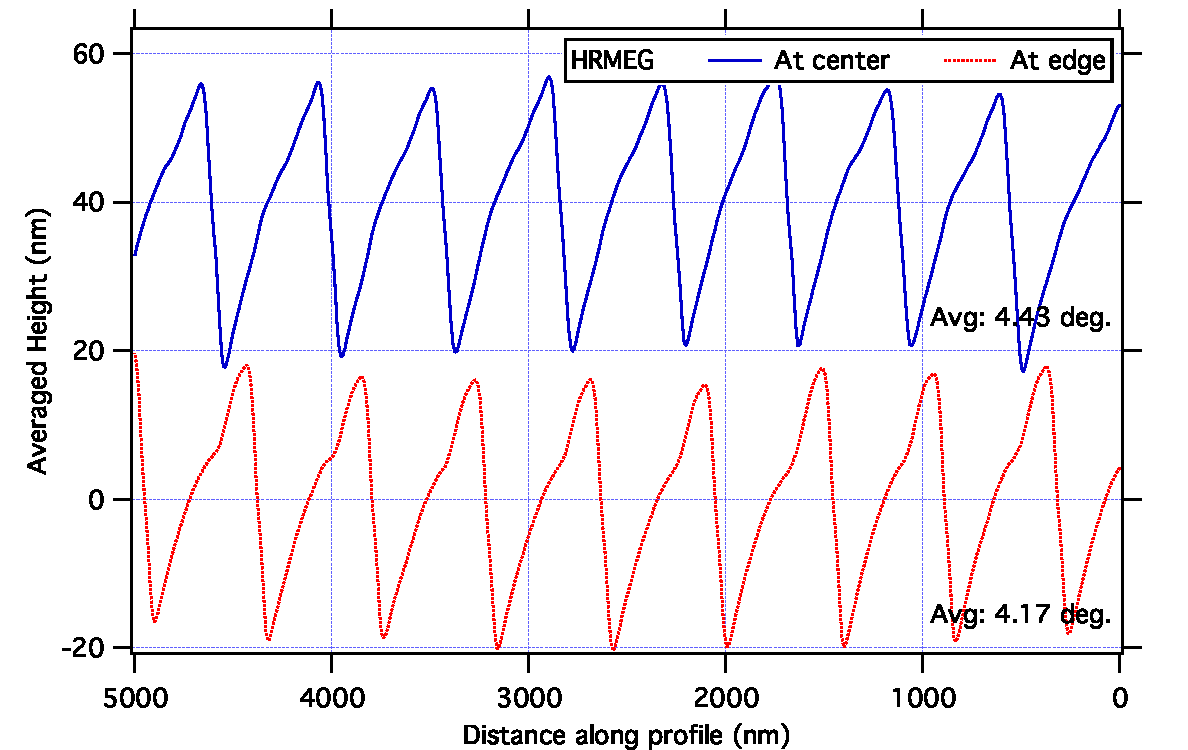
\includegraphics[scale=0.8]{Chapter5/5y_afm/HRMEG.pdf} 
   \caption{AFM measurements of the HighRes Medium Energy Grating (HRMEG) profile, averaged along the grooves (TODO um x TODO um).  The best-fit blaze angle is at the centre of the grating.}
   \label{5y-hrmeg}
\end{figure}

\begin{figure}[htbp] %  figure placement: here, top, bottom, or page
   \centering
   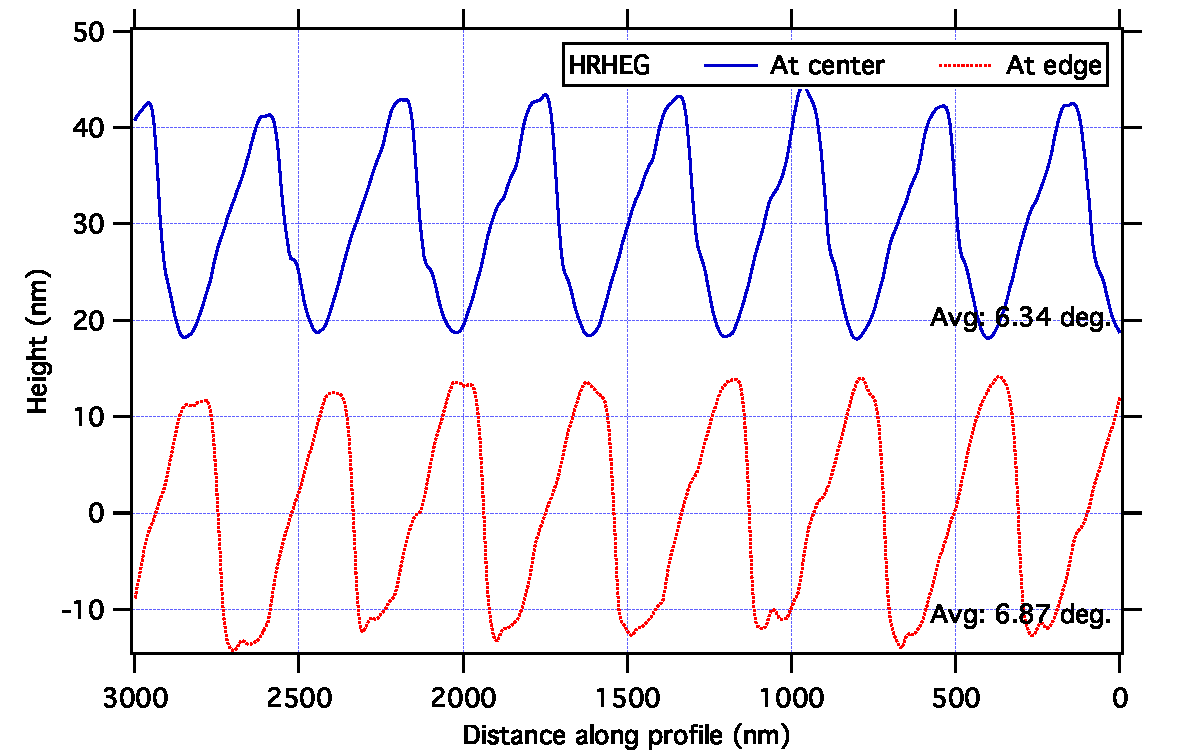
\includegraphics[scale=0.8]{Chapter5/5y_afm/HRHEG.pdf} 
   \caption{AFM measurements of the HighRes High Energy Grating (HRHEG) profile, averaged along the grooves (TODO um x TODO um).  The best-fit blaze angle is at the centre of the grating.}
   \label{5y-hrheg}
\end{figure}




 (Pt): blaze angles very off� Unsuitable for actual application in 3rd order.
          - Temporary plan: Using HRHEG (2600l/mm) in place of HEG (2000l/mm) since blaze angle error makes it suitable for use in 1st order.
               - DATA 5q: plot expected reduction in efficiency
               
